\documentclass[twoside]{book}

% Packages required by doxygen
\usepackage{fixltx2e}
\usepackage{calc}
\usepackage{doxygen}
\usepackage[export]{adjustbox} % also loads graphicx
\usepackage{graphicx}
\usepackage[utf8]{inputenc}
\usepackage{makeidx}
\usepackage{multicol}
\usepackage{multirow}
\PassOptionsToPackage{warn}{textcomp}
\usepackage{textcomp}
\usepackage[nointegrals]{wasysym}
\usepackage[table]{xcolor}

% Font selection
\usepackage[T1]{fontenc}
\usepackage[scaled=.90]{helvet}
\usepackage{courier}
\usepackage{amssymb}
\usepackage{sectsty}
\renewcommand{\familydefault}{\sfdefault}
\allsectionsfont{%
  \fontseries{bc}\selectfont%
  \color{darkgray}%
}
\renewcommand{\DoxyLabelFont}{%
  \fontseries{bc}\selectfont%
  \color{darkgray}%
}
\newcommand{\+}{\discretionary{\mbox{\scriptsize$\hookleftarrow$}}{}{}}

% Page & text layout
\usepackage{geometry}
\geometry{%
  a4paper,%
  top=2.5cm,%
  bottom=2.5cm,%
  left=2.5cm,%
  right=2.5cm%
}
\tolerance=750
\hfuzz=15pt
\hbadness=750
\setlength{\emergencystretch}{15pt}
\setlength{\parindent}{0cm}
\setlength{\parskip}{3ex plus 2ex minus 2ex}
\makeatletter
\renewcommand{\paragraph}{%
  \@startsection{paragraph}{4}{0ex}{-1.0ex}{1.0ex}{%
    \normalfont\normalsize\bfseries\SS@parafont%
  }%
}
\renewcommand{\subparagraph}{%
  \@startsection{subparagraph}{5}{0ex}{-1.0ex}{1.0ex}{%
    \normalfont\normalsize\bfseries\SS@subparafont%
  }%
}
\makeatother

% Headers & footers
\usepackage{fancyhdr}
\pagestyle{fancyplain}
\fancyhead[LE]{\fancyplain{}{\bfseries\thepage}}
\fancyhead[CE]{\fancyplain{}{}}
\fancyhead[RE]{\fancyplain{}{\bfseries\leftmark}}
\fancyhead[LO]{\fancyplain{}{\bfseries\rightmark}}
\fancyhead[CO]{\fancyplain{}{}}
\fancyhead[RO]{\fancyplain{}{\bfseries\thepage}}
\fancyfoot[LE]{\fancyplain{}{}}
\fancyfoot[CE]{\fancyplain{}{}}
\fancyfoot[RE]{\fancyplain{}{\bfseries\scriptsize Generated by Doxygen }}
\fancyfoot[LO]{\fancyplain{}{\bfseries\scriptsize Generated by Doxygen }}
\fancyfoot[CO]{\fancyplain{}{}}
\fancyfoot[RO]{\fancyplain{}{}}
\renewcommand{\footrulewidth}{0.4pt}
\renewcommand{\chaptermark}[1]{%
  \markboth{#1}{}%
}
\renewcommand{\sectionmark}[1]{%
  \markright{\thesection\ #1}%
}

% Indices & bibliography
\usepackage{natbib}
\usepackage[titles]{tocloft}
\setcounter{tocdepth}{3}
\setcounter{secnumdepth}{5}
\makeindex

% Custom commands
\newcommand{\clearemptydoublepage}{%
  \newpage{\pagestyle{empty}\cleardoublepage}%
}

\usepackage{caption}
\captionsetup{labelsep=space,justification=centering,font={bf},singlelinecheck=off,skip=4pt,position=top}

%===== C O N T E N T S =====

\begin{document}

% Titlepage & ToC
\pagenumbering{alph}
\begin{titlepage}
\vspace*{7cm}
\begin{center}%
{\Large Movie Guide Application }\\
\vspace*{1cm}
{\large Generated by Doxygen 1.8.14}\\
\end{center}
\end{titlepage}
\clearemptydoublepage
\pagenumbering{roman}
\tableofcontents
\clearemptydoublepage
\pagenumbering{arabic}

%--- Begin generated contents ---
\chapter{Hierarchical Index}
\section{Class Hierarchy}
This inheritance list is sorted roughly, but not completely, alphabetically\+:\begin{DoxyCompactList}
\item \contentsline{section}{movieguideapplication.\+Api\+Utils}{\pageref{classmovieguideapplication_1_1_api_utils}}{}
\item \contentsline{section}{movieguideapplication.\+Movie}{\pageref{classmovieguideapplication_1_1_movie}}{}
\item \contentsline{section}{movieguideapplication.\+Movie\+List}{\pageref{classmovieguideapplication_1_1_movie_list}}{}
\item \contentsline{section}{movieguideapplication.\+Movie\+Retriever}{\pageref{interfacemovieguideapplication_1_1_movie_retriever}}{}
\item \contentsline{section}{movieguideapplication.\+Retrofit\+Client}{\pageref{classmovieguideapplication_1_1_retrofit_client}}{}
\item App\+Compat\+Activity\begin{DoxyCompactList}
\item \contentsline{section}{movieguideapplication.\+Main\+Activity}{\pageref{classmovieguideapplication_1_1_main_activity}}{}
\end{DoxyCompactList}
\end{DoxyCompactList}

\chapter{Class Index}
\section{Class List}
Here are the classes, structs, unions and interfaces with brief descriptions\+:\begin{DoxyCompactList}
\item\contentsline{section}{\textbf{ movieguideapplication.\+Api\+Utils} }{\pageref{classmovieguideapplication_1_1_api_utils}}{}
\item\contentsline{section}{\textbf{ movieguideapplication.\+Main\+Activity} }{\pageref{classmovieguideapplication_1_1_main_activity}}{}
\item\contentsline{section}{\textbf{ movieguideapplication.\+Movie} }{\pageref{classmovieguideapplication_1_1_movie}}{}
\item\contentsline{section}{\textbf{ movieguideapplication.\+Movie\+List} }{\pageref{classmovieguideapplication_1_1_movie_list}}{}
\item\contentsline{section}{\textbf{ movieguideapplication.\+Movie\+Retriever} }{\pageref{interfacemovieguideapplication_1_1_movie_retriever}}{}
\item\contentsline{section}{\textbf{ movieguideapplication.\+Retrofit\+Client} }{\pageref{classmovieguideapplication_1_1_retrofit_client}}{}
\end{DoxyCompactList}

\chapter{Class Documentation}
\section{movieguideapplication.\+Api\+Utils Class Reference}
\label{classmovieguideapplication_1_1_api_utils}\index{movieguideapplication.\+Api\+Utils@{movieguideapplication.\+Api\+Utils}}
\subsection*{Static Public Member Functions}
\begin{DoxyCompactItemize}
\item 
static \textbf{ Movie\+Retriever} \textbf{ get\+Movie\+Retirever} ()
\end{DoxyCompactItemize}
\subsection*{Static Public Attributes}
\begin{DoxyCompactItemize}
\item 
static final String \textbf{ B\+A\+S\+E\+\_\+\+U\+RL} = \char`\"{}http\+://api.\+themoviedb.\+org\char`\"{}
\end{DoxyCompactItemize}


\subsection{Detailed Description}
A\+PI Utils Class This class primes the U\+RL for a get request to be made using the Retrofit client 

\subsection{Member Function Documentation}
\mbox{\label{classmovieguideapplication_1_1_api_utils_a0fd680c99a77e09755e56e4ad3c9ce51}} 
\index{movieguideapplication\+::\+Api\+Utils@{movieguideapplication\+::\+Api\+Utils}!get\+Movie\+Retirever@{get\+Movie\+Retirever}}
\index{get\+Movie\+Retirever@{get\+Movie\+Retirever}!movieguideapplication\+::\+Api\+Utils@{movieguideapplication\+::\+Api\+Utils}}
\subsubsection{get\+Movie\+Retirever()}
{\footnotesize\ttfamily static \textbf{ Movie\+Retriever} movieguideapplication.\+Api\+Utils.\+get\+Movie\+Retirever (\begin{DoxyParamCaption}{ }\end{DoxyParamCaption})\hspace{0.3cm}{\ttfamily [static]}}

This method creates an object of the \doxyref{Movie\+Retriever}{p.}{interfacemovieguideapplication_1_1_movie_retriever} class using the Retrofit Client \begin{DoxyReturn}{Returns}
A \doxyref{Movie\+Retriever}{p.}{interfacemovieguideapplication_1_1_movie_retriever} object using the B\+A\+S\+E\+\_\+\+U\+RL variable 
\end{DoxyReturn}


\subsection{Member Data Documentation}
\mbox{\label{classmovieguideapplication_1_1_api_utils_a0b060f2992d06e99681fb8ae1f53f3a1}} 
\index{movieguideapplication\+::\+Api\+Utils@{movieguideapplication\+::\+Api\+Utils}!B\+A\+S\+E\+\_\+\+U\+RL@{B\+A\+S\+E\+\_\+\+U\+RL}}
\index{B\+A\+S\+E\+\_\+\+U\+RL@{B\+A\+S\+E\+\_\+\+U\+RL}!movieguideapplication\+::\+Api\+Utils@{movieguideapplication\+::\+Api\+Utils}}
\subsubsection{B\+A\+S\+E\+\_\+\+U\+RL}
{\footnotesize\ttfamily final String movieguideapplication.\+Api\+Utils.\+B\+A\+S\+E\+\_\+\+U\+RL = \char`\"{}http\+://api.\+themoviedb.\+org\char`\"{}\hspace{0.3cm}{\ttfamily [static]}}

The U\+RL to which the A\+PI get request will be made 

The documentation for this class was generated from the following file\+:\begin{DoxyCompactItemize}
\item 
Api\+Utils.\+java\end{DoxyCompactItemize}

\section{movieguideapplication.\+Main\+Activity Class Reference}
\label{classmovieguideapplication_1_1_main_activity}\index{movieguideapplication.\+Main\+Activity@{movieguideapplication.\+Main\+Activity}}
Inheritance diagram for movieguideapplication.\+Main\+Activity\+:\begin{figure}[H]
\begin{center}
\leavevmode
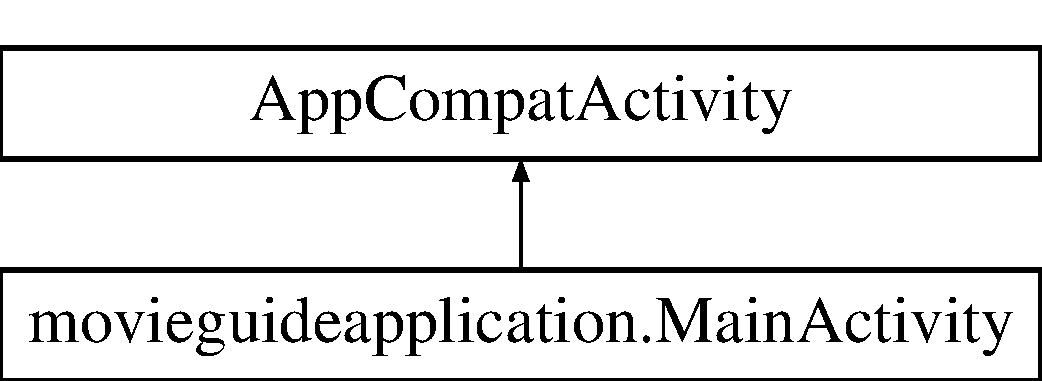
\includegraphics[height=2.000000cm]{classmovieguideapplication_1_1_main_activity}
\end{center}
\end{figure}
\subsection*{Protected Member Functions}
\begin{DoxyCompactItemize}
\item 
void \textbf{ on\+Create} (Bundle saved\+Instance\+State)
\end{DoxyCompactItemize}


\subsection{Detailed Description}
Parent class of the application 

\subsection{Member Function Documentation}
\mbox{\label{classmovieguideapplication_1_1_main_activity_a0e3b9ebf18a76a620b61408101b0de96}} 
\index{movieguideapplication\+::\+Main\+Activity@{movieguideapplication\+::\+Main\+Activity}!on\+Create@{on\+Create}}
\index{on\+Create@{on\+Create}!movieguideapplication\+::\+Main\+Activity@{movieguideapplication\+::\+Main\+Activity}}
\subsubsection{on\+Create()}
{\footnotesize\ttfamily void movieguideapplication.\+Main\+Activity.\+on\+Create (\begin{DoxyParamCaption}\item[{Bundle}]{saved\+Instance\+State }\end{DoxyParamCaption})\hspace{0.3cm}{\ttfamily [protected]}}

Creates the user interface when the application is run 
\begin{DoxyParams}{Parameters}
{\em saved\+Instance\+State} & Holds the saved state of the application \\
\hline
\end{DoxyParams}


The documentation for this class was generated from the following file\+:\begin{DoxyCompactItemize}
\item 
Main\+Activity.\+java\end{DoxyCompactItemize}

\section{movieguideapplication.\+Movie Class Reference}
\label{classmovieguideapplication_1_1_movie}\index{movieguideapplication.\+Movie@{movieguideapplication.\+Movie}}
\subsection*{Public Member Functions}
\begin{DoxyCompactItemize}
\item 
String \textbf{ get\+Title} ()
\item 
\textbf{ Movie} (int id, boolean video, double vote\+\_\+average, String title, double popularity)
\end{DoxyCompactItemize}


\subsection{Detailed Description}
Parses data extracted from the A\+PI 

\subsection{Constructor \& Destructor Documentation}
\mbox{\label{classmovieguideapplication_1_1_movie_ad97e0d1d039f5be047adfcba2a9d030f}} 
\index{movieguideapplication\+::\+Movie@{movieguideapplication\+::\+Movie}!Movie@{Movie}}
\index{Movie@{Movie}!movieguideapplication\+::\+Movie@{movieguideapplication\+::\+Movie}}
\subsubsection{Movie()}
{\footnotesize\ttfamily movieguideapplication.\+Movie.\+Movie (\begin{DoxyParamCaption}\item[{int}]{id,  }\item[{boolean}]{video,  }\item[{double}]{vote\+\_\+average,  }\item[{String}]{title,  }\item[{double}]{popularity }\end{DoxyParamCaption})}

Constructor for the \doxyref{Movie}{p.}{classmovieguideapplication_1_1_movie} Class 
\begin{DoxyParams}{Parameters}
{\em id} & Contains the ID number of the movie \\
\hline
{\em video} & Boolean value corresponding to the availability of the movie trailer \\
\hline
{\em vote\+\_\+average} & Contains the average rating of the movie \\
\hline
{\em title} & Contains a numerical value for the popularity of the movie \\
\hline
{\em popularity} & Contains a numerical value for the popularity of the movie \\
\hline
\end{DoxyParams}


\subsection{Member Function Documentation}
\mbox{\label{classmovieguideapplication_1_1_movie_a721a3459fe03eb3f1c3ded7b6dfb0955}} 
\index{movieguideapplication\+::\+Movie@{movieguideapplication\+::\+Movie}!get\+Title@{get\+Title}}
\index{get\+Title@{get\+Title}!movieguideapplication\+::\+Movie@{movieguideapplication\+::\+Movie}}
\subsubsection{get\+Title()}
{\footnotesize\ttfamily String movieguideapplication.\+Movie.\+get\+Title (\begin{DoxyParamCaption}{ }\end{DoxyParamCaption})}

Gets the title of the movie \begin{DoxyReturn}{Returns}
string containing the title 
\end{DoxyReturn}


The documentation for this class was generated from the following file\+:\begin{DoxyCompactItemize}
\item 
Movie.\+java\end{DoxyCompactItemize}

\section{movieguideapplication.\+Movie\+List Class Reference}
\label{classmovieguideapplication_1_1_movie_list}\index{movieguideapplication.\+Movie\+List@{movieguideapplication.\+Movie\+List}}
\subsection*{Public Member Functions}
\begin{DoxyCompactItemize}
\item 
List$<$ \textbf{ Movie} $>$ \textbf{ get\+Movies} ()
\item 
void \textbf{ set\+Movies} (List$<$ \textbf{ Movie} $>$ movies)
\end{DoxyCompactItemize}


\subsection{Detailed Description}
Contains getter and setter methods for the list of movies loaded from the A\+PI 

\subsection{Member Function Documentation}
\mbox{\label{classmovieguideapplication_1_1_movie_list_a9bf964c6de477d41c348973ff3499744}} 
\index{movieguideapplication\+::\+Movie\+List@{movieguideapplication\+::\+Movie\+List}!get\+Movies@{get\+Movies}}
\index{get\+Movies@{get\+Movies}!movieguideapplication\+::\+Movie\+List@{movieguideapplication\+::\+Movie\+List}}
\subsubsection{get\+Movies()}
{\footnotesize\ttfamily List$<$\textbf{ Movie}$>$ movieguideapplication.\+Movie\+List.\+get\+Movies (\begin{DoxyParamCaption}{ }\end{DoxyParamCaption})}

Gets the list of loaded movies \begin{DoxyReturn}{Returns}
list of movies loaded from A\+PI 
\end{DoxyReturn}
\mbox{\label{classmovieguideapplication_1_1_movie_list_a191cca47a9510755f460ebe137279234}} 
\index{movieguideapplication\+::\+Movie\+List@{movieguideapplication\+::\+Movie\+List}!set\+Movies@{set\+Movies}}
\index{set\+Movies@{set\+Movies}!movieguideapplication\+::\+Movie\+List@{movieguideapplication\+::\+Movie\+List}}
\subsubsection{set\+Movies()}
{\footnotesize\ttfamily void movieguideapplication.\+Movie\+List.\+set\+Movies (\begin{DoxyParamCaption}\item[{List$<$ \textbf{ Movie} $>$}]{movies }\end{DoxyParamCaption})}

Updates the list of movies 
\begin{DoxyParams}{Parameters}
{\em movies} & new list of movies \\
\hline
\end{DoxyParams}


The documentation for this class was generated from the following file\+:\begin{DoxyCompactItemize}
\item 
Movie\+List.\+java\end{DoxyCompactItemize}

\section{movieguideapplication.\+Movie\+Retriever Interface Reference}
\label{interfacemovieguideapplication_1_1_movie_retriever}\index{movieguideapplication.\+Movie\+Retriever@{movieguideapplication.\+Movie\+Retriever}}
\subsection*{Public Member Functions}
\begin{DoxyCompactItemize}
\item 
Call$<$ \textbf{ Movie\+List} $>$ \textbf{ get\+Movies} ()
\item 
Call$<$ \textbf{ Movie\+List} $>$ \textbf{ get\+Movies} (@Query(\char`\"{}page\char`\"{}) int page)
\end{DoxyCompactItemize}


\subsection{Detailed Description}
Makes get requests to the A\+PI using the Retrofit Client annotations 

\subsection{Member Function Documentation}
\mbox{\label{interfacemovieguideapplication_1_1_movie_retriever_a2f5c95d2cfb882c13b914994fd722ff0}} 
\index{movieguideapplication\+::\+Movie\+Retriever@{movieguideapplication\+::\+Movie\+Retriever}!get\+Movies@{get\+Movies}}
\index{get\+Movies@{get\+Movies}!movieguideapplication\+::\+Movie\+Retriever@{movieguideapplication\+::\+Movie\+Retriever}}
\subsubsection{get\+Movies()\hspace{0.1cm}{\footnotesize\ttfamily [1/2]}}
{\footnotesize\ttfamily Call$<$\textbf{ Movie\+List}$>$ movieguideapplication.\+Movie\+Retriever.\+get\+Movies (\begin{DoxyParamCaption}{ }\end{DoxyParamCaption})}

Get request for movies based by popularity \begin{DoxyReturn}{Returns}
list of call responses from the A\+PI 
\end{DoxyReturn}
\mbox{\label{interfacemovieguideapplication_1_1_movie_retriever_a5340c26b91170dc7aa275847cee41dbc}} 
\index{movieguideapplication\+::\+Movie\+Retriever@{movieguideapplication\+::\+Movie\+Retriever}!get\+Movies@{get\+Movies}}
\index{get\+Movies@{get\+Movies}!movieguideapplication\+::\+Movie\+Retriever@{movieguideapplication\+::\+Movie\+Retriever}}
\subsubsection{get\+Movies()\hspace{0.1cm}{\footnotesize\ttfamily [2/2]}}
{\footnotesize\ttfamily Call$<$\textbf{ Movie\+List}$>$ movieguideapplication.\+Movie\+Retriever.\+get\+Movies (\begin{DoxyParamCaption}\item[{@Query(\char`\"{}page\char`\"{}) int}]{page }\end{DoxyParamCaption})}

Get request for movies based by popularity and specified page 
\begin{DoxyParams}{Parameters}
{\em page} & Page to extract movies from \\
\hline
\end{DoxyParams}
\begin{DoxyReturn}{Returns}
list of call responses from the A\+PI 
\end{DoxyReturn}


The documentation for this interface was generated from the following file\+:\begin{DoxyCompactItemize}
\item 
Movie\+Retriever.\+java\end{DoxyCompactItemize}

\section{movieguideapplication.\+Retrofit\+Client Class Reference}
\label{classmovieguideapplication_1_1_retrofit_client}\index{movieguideapplication.\+Retrofit\+Client@{movieguideapplication.\+Retrofit\+Client}}
\subsection*{Static Public Member Functions}
\begin{DoxyCompactItemize}
\item 
static Retrofit \textbf{ get\+Client} (String base\+Url)
\end{DoxyCompactItemize}


\subsection{Detailed Description}
Setup for the \doxyref{Retrofit\+Client}{p.}{classmovieguideapplication_1_1_retrofit_client} 

\subsection{Member Function Documentation}
\mbox{\label{classmovieguideapplication_1_1_retrofit_client_a9d61e0a94ccc0a061fa68c0dd91c935e}} 
\index{movieguideapplication\+::\+Retrofit\+Client@{movieguideapplication\+::\+Retrofit\+Client}!get\+Client@{get\+Client}}
\index{get\+Client@{get\+Client}!movieguideapplication\+::\+Retrofit\+Client@{movieguideapplication\+::\+Retrofit\+Client}}
\subsubsection{get\+Client()}
{\footnotesize\ttfamily static Retrofit movieguideapplication.\+Retrofit\+Client.\+get\+Client (\begin{DoxyParamCaption}\item[{String}]{base\+Url }\end{DoxyParamCaption})\hspace{0.3cm}{\ttfamily [static]}}

Provides framework for retrofit object 
\begin{DoxyParams}{Parameters}
{\em base\+Url} & The U\+RL to which a get request will be made \\
\hline
\end{DoxyParams}
\begin{DoxyReturn}{Returns}
retrofit object 
\end{DoxyReturn}


The documentation for this class was generated from the following file\+:\begin{DoxyCompactItemize}
\item 
Retrofit\+Client.\+java\end{DoxyCompactItemize}

%--- End generated contents ---

% Index
\backmatter
\newpage
\phantomsection
\clearemptydoublepage
\addcontentsline{toc}{chapter}{Index}
\printindex

\end{document}
